% Created 2023-10-13 Fri 20:54
% Intended LaTeX compiler: pdflatex
\documentclass[11pt]{article}
\usepackage[utf8]{inputenc}
\usepackage[T1]{fontenc}
\usepackage{graphicx}
\usepackage{longtable}
\usepackage{wrapfig}
\usepackage{rotating}
\usepackage[normalem]{ulem}
\usepackage{amsmath}
\usepackage{amssymb}
\usepackage{capt-of}
\usepackage{hyperref}
\notindent \notag  \usepackage{amsmath} \usepackage[a4paper,margin=1in,portrait]{geometry}
\author{Elizabeth Hunt}
\date{\today}
\title{Homework 4}
\hypersetup{
 pdfauthor={Elizabeth Hunt},
 pdftitle={Homework 4},
 pdfkeywords={},
 pdfsubject={},
 pdfcreator={Emacs 28.2 (Org mode 9.7-pre)}, 
 pdflang={English}}
\begin{document}

\maketitle
\setlength\parindent{0pt}

\section{Question 1}
\label{sec:org0ce46da}
See the attached LIZFCM Software Manual.

\section{Question 2, 3, 4}
\label{sec:org0794d50}
\begin{center}
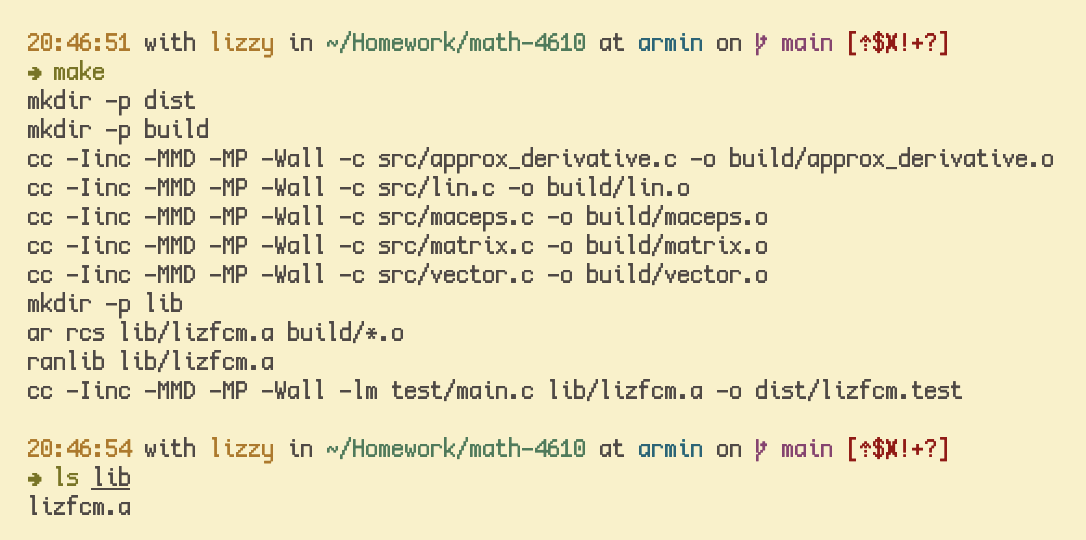
\includegraphics[width=350px]{./img/make_run.png}
\end{center}

\section{Question 5}
\label{sec:orgf7b84cc}
\begin{center}
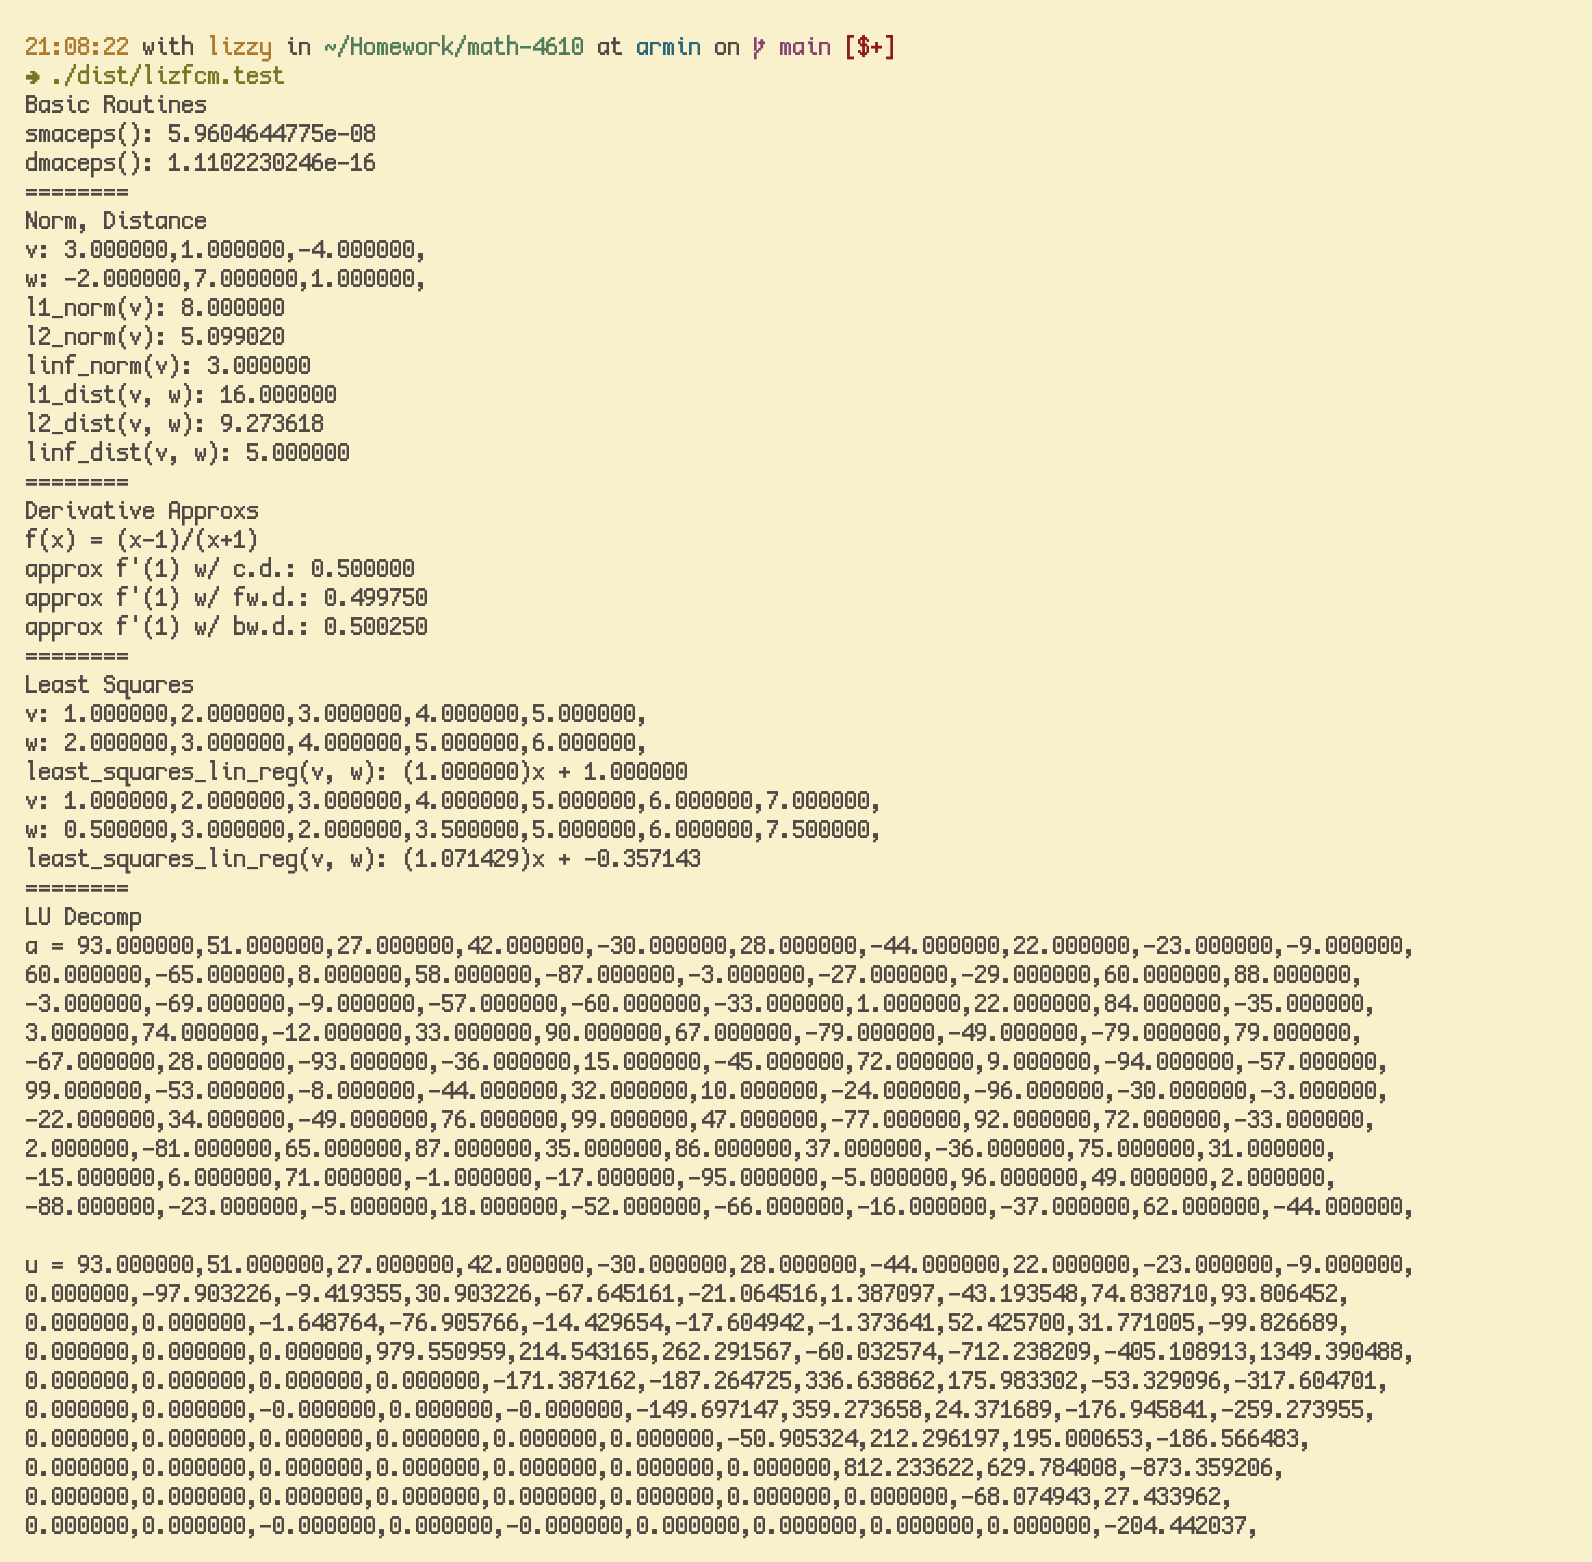
\includegraphics[width=350px]{./img/test_routine_1.png}
\end{center}

\begin{center}
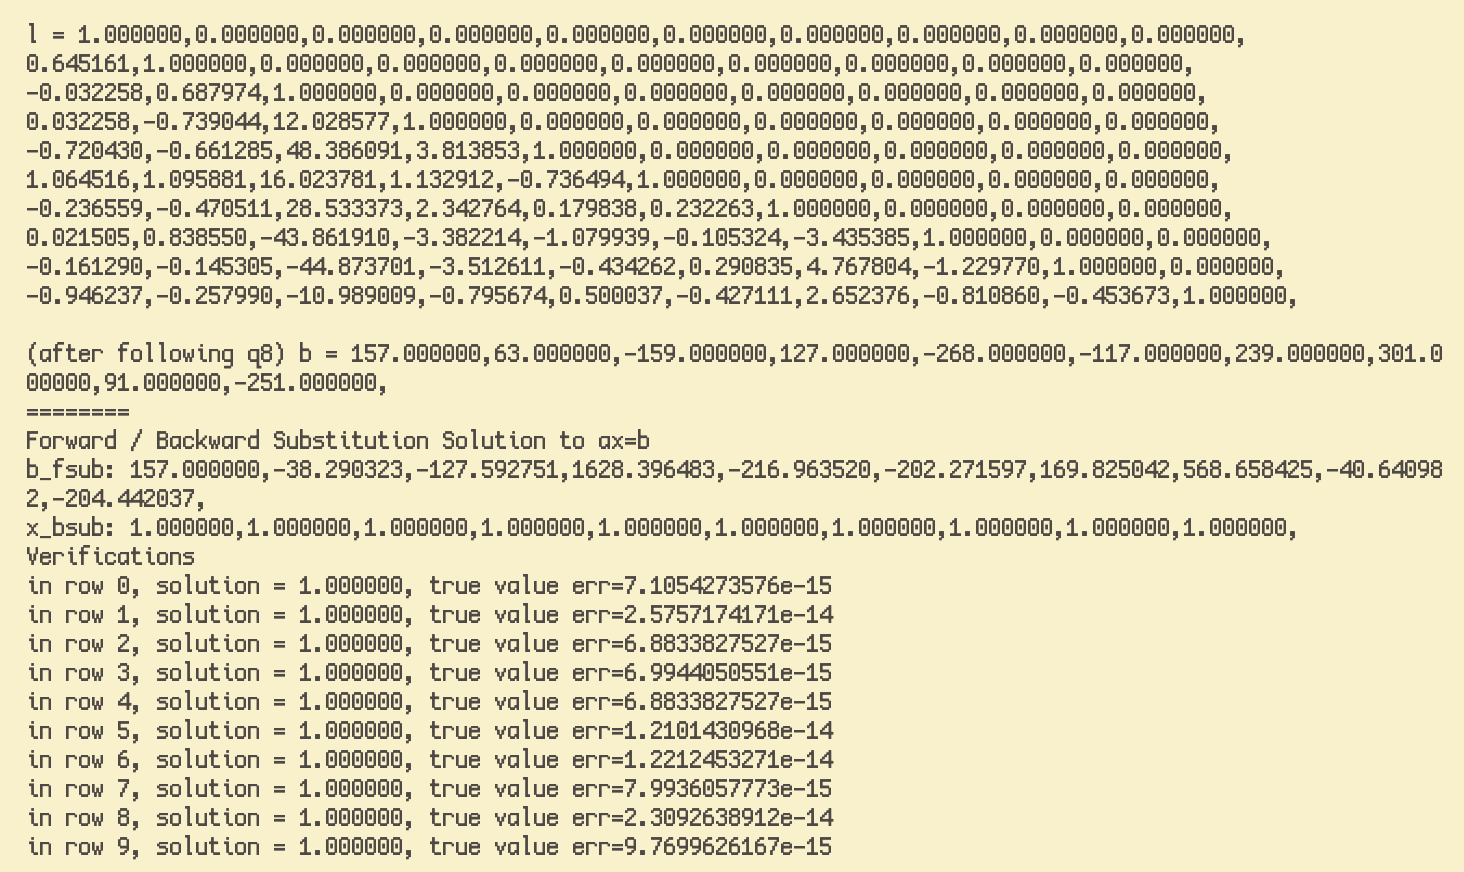
\includegraphics[width=350px]{./img/test_routine_2.png}
\end{center}

\section{Question 6}
\label{sec:orgee1884d}
See the LIZFCM Software Manual.

\section{Question 7}
\label{sec:org6f86e09}
See \texttt{src/matrix.c -> lu\_decomp, fsubst, bsubst, solve\_matrix}

\section{Question 8}
\label{sec:orga79c31e}
See \texttt{test/main.c -> lines 109 - 113} in correspondence to the run in Question 5

\section{Question 9}
\label{sec:org5b1b74d}
See \texttt{test/main.c -> lines 118 - 121} in correspondence to the run in Question 5

\section{Question 10}
\label{sec:org7409683}
See the TOC on the first page of the LIZFCM Software Manual.
\end{document}